\section{Informal Logic Proof}

\subsection{ No Repeat }

\subsection{ 狹義的 statement }
重述一次 the statement we have to proof:
``Given a reversible abstract machine, it will inevitably terminate from any initial state with a finite number of total states.''

Here is the graph of the machine we expected.  It seems monotonous.  The initial state will 不重複地 經過 all the other states and then terminate.

\vspace{1em}

\usetikzlibrary{graphs, positioning, quotes, shapes.geometric}

\begin{document}
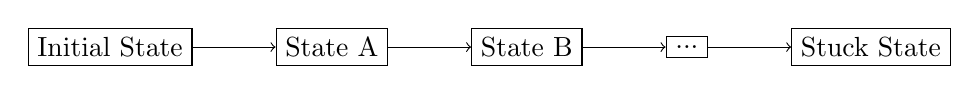
\begin{tikzpicture}[node distance=10pt]
    \node[draw]                           (State 0)  {Initial State};
    \node[draw, right=30pt of State 0]    (State 1)  {State A};
    \node[draw, right=30pt of State 1]    (State 2)  {State B};
    \node[draw, right=30pt of State 2]    (State 3)  {...};
    \node[draw, right=30pt of State 3]    (State 4)  {Stuck State};
    
    \graph{
        (State 0) -> (State 1) -> (State 2) -> (State 3) -> (State 4);
    };
\end{tikzpicture}

This is the other case for the machine with finite states.  In the graph, the initial state also walk through finite state and terminate.  However, not all the states are traversed.

\vspace{1em}

\usetikzlibrary{graphs, positioning, quotes, shapes.geometric}

\begin{document}
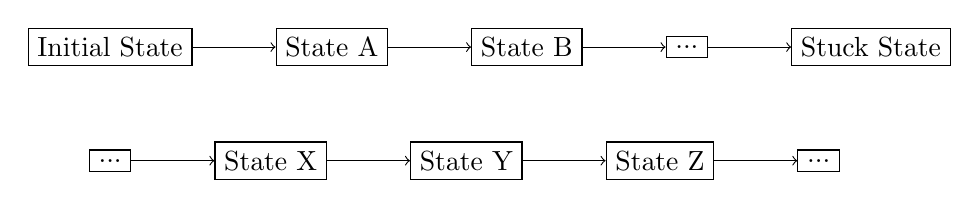
\begin{tikzpicture}[node distance=10pt]
    \node[draw]                           (State 0)  {Initial State};
    \node[draw, right=30pt of State 0]    (State 1)  {State A};
    \node[draw, right=30pt of State 1]    (State 2)  {State B};
    \node[draw, right=30pt of State 2]    (State 3)  {...};
    \node[draw, right=30pt of State 3]    (State 4)  {Stuck State};

    \node[draw, below=30pt of State 0]     (State 5)  {...};
    \node[draw, right=30pt of State 5]     (State 6)  {State X};
    \node[draw, right=30pt of State 6]     (State 7)  {State Y};
    \node[draw, right=30pt of State 7]     (State 8)  {State Z};
    \node[draw, right=30pt of State 8]     (State 9)  {...};
    
    \graph{
        (State 0) -> (State 1) -> (State 2) -> (State 3) -> (State 4);
        (State 5) -> (State 6) -> (State 7) -> (State 8) -> (State 9);
    };
\end{tikzpicture}


Assume number of all states is N.  That is, we have $st_{0}$, $st_{1}$, ..., and $st_{N-1}$.
Assume $st_{0}$ is the initial state, we can check whether $st_{0}$ has next state.
Once current state doesn't have next state, the machine will terminate.  
Therefore, we just have to consider the states starting from $st_{0}$ always have its next state.

當 trace 推移了 N 次, it should be like the graph below:

\vspace{1em}

\usetikzlibrary{graphs, positioning, quotes, shapes.geometric}

\begin{document}
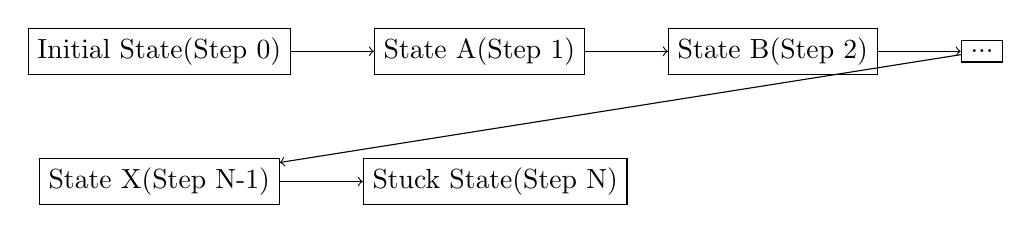
\begin{tikzpicture}[node distance=10pt]
    \node[draw]                           (State 0)  {Initial State(Step 0)};
    \node[draw, right=30pt of State 0]    (State 1)  {State A(Step 1)};
    \node[draw, right=30pt of State 1]    (State 2)  {State B(Step 2)};
    \node[draw, right=30pt of State 2]    (State 3)  {...};
    \node[draw, below=30pt of State 0]    (State 4)  {State X(Step N-1)};
    \node[draw, right=30pt of State 4]    (State 5)  {Stuck State(Step N)};
    
    \graph{
        (State 0) -> (State 1) -> (State 2) -> (State 3) -> (State 4) -> (State 5);
    };
\end{tikzpicture}

這裡,我們不特別提及已遍歷的前n個state應完全不重複,即使顯而易見地他們重複時會引發矛盾。
我們將重點關注於 the whole trace with lenth of N+1.
The reversible machine have only N states, but there are N+1 state we have traversed.
According to piegonhole principle, we can find two same states in the trace.

\vspace{1em}

\usetikzlibrary{graphs, positioning, quotes, shapes.geometric}

\begin{document}
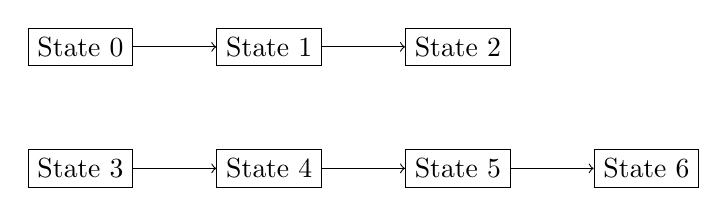
\begin{tikzpicture}[node distance=10pt]
    % 單純一條線,從initial state 到 finite state
    \node[draw]                           (State 0)  {State 0};
    \node[draw, right=30pt of State 0]    (State 1)  {State 1};
    \node[draw, right=30pt of State 1]    (State 2)  {State 2};
    
    \node[draw, below=30pt of State 0]    (State 3)  {State 3};
    \node[draw, right=30pt of State 3]    (State 4)  {State 4};
    \node[draw, right=30pt of State 4]    (State 5)  {State 5};
    \node[draw, right=30pt of State 5]    (State 6)  {State 6};

    \graph{
        (State 0) -> (State 1) -> (State 2);
        (State 3) -> (State 4) -> (State 5) -> (State 6);
    };
\end{tikzpicture}

With No-Repeat principle, we know it's impossible for an initial state, walk through two different steps but reach same state.
到這邊,我們成功找出矛盾。 The contradiction shows the length of trace is always less or equal than N, and then terminate.

\subsection{ 廣義的 statement }
Similar to Narrow RevTerminate Principle, we assume $st_{0}$ is the $$initial state, and 關注於 there are always states after each state we walk through.
The Broad RevTerminate Principle says there is only N states $st_{0}$ can reach.  我們與先前一樣走N步以讓the length of trace be N+1.

\vspace{1em}

\usetikzlibrary{graphs, positioning, quotes, shapes.geometric}

\begin{document}
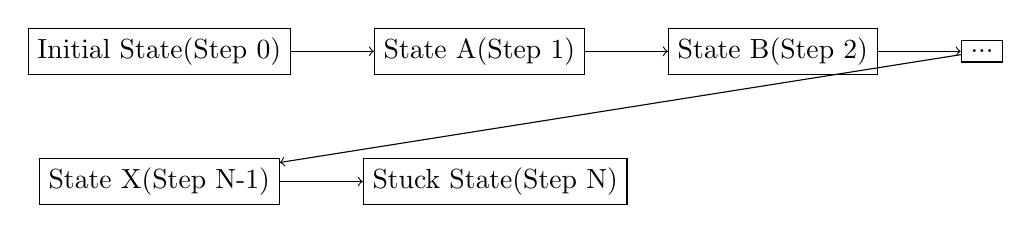
\begin{tikzpicture}[node distance=10pt]
    \node[draw]                           (State 0)  {Initial State(Step 0)};
    \node[draw, right=30pt of State 0]    (State 1)  {State A(Step 1)};
    \node[draw, right=30pt of State 1]    (State 2)  {State B(Step 2)};
    \node[draw, right=30pt of State 2]    (State 3)  {...};
    \node[draw, below=30pt of State 0]    (State 4)  {State X(Step N-1)};
    \node[draw, right=30pt of State 4]    (State 5)  {Stuck State(Step N)};
    
    \graph{
        (State 0) -> (State 1) -> (State 2) -> (State 3) -> (State 4) -> (State 5);
    };
\end{tikzpicture}

